% !TeX document-id = {5c05c331-134f-48f1-8db3-fd32c67a647b}
%%%%%%%%%%%%%%%%%%%%%%%%%%%%%%%%%%%%%%%%%
% Journal Article
% LaTeX Template
% Version 2.0 (February 7, 2023)
%
% This template originates from:
% https://www.LaTeXTemplates.com
%
% Author:
% Vel (vel@latextemplates.com)
%
% License:
% CC BY-NC-SA 4.0 (https://creativecommons.org/licenses/by-nc-sa/4.0/)
%
% NOTE: The bibliography needs to be compiled using the biber engine.
%
%%%%%%%%%%%%%%%%%%%%%%%%%%%%%%%%%%%%%%%%%

% Magic comments for TeXStudio
% !TeX program = pdflatex
% !BIB program = biber
% !TeX encoding = utf8
% !TeX spellcheck = en_US
%----------------------------------------------------------------------------------------
%	ARTICLE CONTENTS
%----------------------------------------------------------------------------------------
\section{Lecture 1 - Signals and Systems}
\subsection{What is a signal?}
Variations of a physical quantity that can be manipulated, stored, or transmitted by physical processes. It is a function of time and space!
\newline Mathematical representation of signals (1D, 2D):
\begin{itemize}
	\item Continuous time signal $x(t), p(x,y)$
	\item Discrete time signal $x[n] = x[nT_s], p[m,n] = p[m\Delta_x ,n\Delta_y] $ with $T_s$ and $\Delta_x$, $\Delta_y$ being the sampling period
\end{itemize}
\subsection{What is a system?}
Something that can manipulate, change, record, or transmit signals. Systems operate on signals to produce new signals or new signal representations.
\newline A sampler is defined as a system whose input is a continuous-time signal x(t) and whose output is the corresponding sequence of samples, defined by the equation x[n] = x(nT) which simply states that the sampler “takes an instantaneous snapshot” of the continuous- time input signal once every T seconds.
\subsection{Sinusoids}
They are the basic building blocks of signals and systems. General formula:
\begin{equation}
	x(t)=A \cos(\omega_0 t+\varphi)=A \cos(2\pi f_0 t+\varphi)
\end{equation}
with $A$ the amplitude, $\omega_0$ the radian frequency, $f_0$ the cyclic frequency, the period $T_0 = \dfrac{2 \pi}{\omega_0} = \dfrac{1}{f_0}$ and $\varphi$ the phase.
\newline A tuning fork is a very simple and familiar system for generating a sinusoidal signal.
\subsection{Review of Sine and Cosine Functions}
\begin{figure}[h]
	\centering
	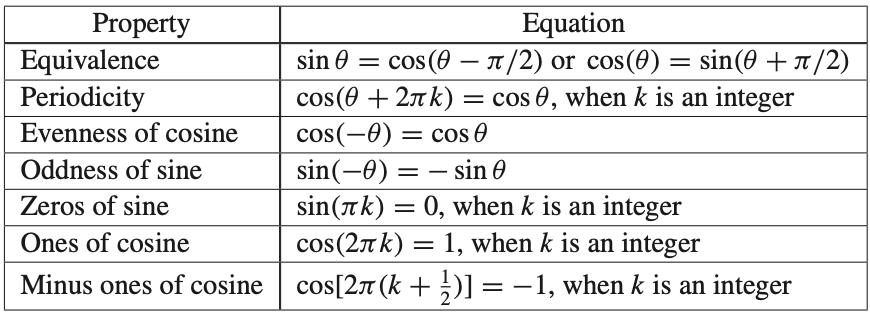
\includegraphics[width=0.7\linewidth]{Figures/DSP_Figures_Lecture1/Basic_Properties_SinCosine}
	\caption{Basic properties of the sine and cosine functions}
	\label{fig:basicpropertiessincosine}
\end{figure}
\begin{figure}[h]
	\centering
	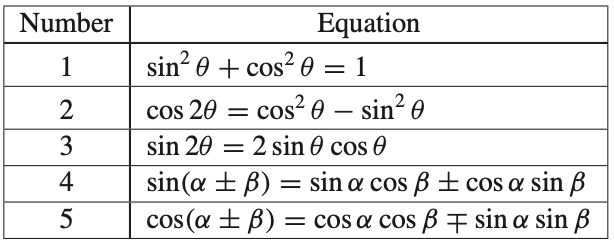
\includegraphics[scale=0.80]{Figures/DSP_Figures_Lecture1/Trigonometric_Identities}
	\caption{Some basic trigonometric identities}
	\label{fig:trigonometric_identities}
\end{figure}
\subsection{Time and Phase Shift}
Time-shifting
\begin{itemize}
	\item Whenever a signal can be expressed in the form $x_1 (t) = s(t - t_1)$, we say that $x_1 (t)$ is a time-shifted version of $s(t)$. If $t_1$ is a positive number, then the shift is to the right, and we say that the signal $s(t)$ has been delayed in time. When $t_1$ is a negative number, then the shift is to the left, and we say that the signal $s(t)$ was advanced in time.
\end{itemize}
Phase shift
\begin{itemize}
	\item The phase parameter $\varphi$ (together with the frequency) determines the time locations of the maxima and minima of a cosine wave, as well as the zero crossings in-between. We can relate the time delay to phase.
	\item Let $x_0 (t) = A \cos(\omega_0 t)$ denote a cosine signal with zero phase. A delay of $x_0 (t)$ can be converted to a phase $\varphi$ by making the following comparison:
	\begin{equation}
		x_0 (t - t_1 ) = A \cos(\omega_0 (t - t_1 )) = A \cos(\omega_0 t + \varphi)
	\end{equation}
	with $\varphi=-\omega_0 t_1$. Notice that the phase is negative when the time shift $t_1$ is positive (a delay)
	\item We can also express the phase in terms of the period $T_0 = \dfrac{1}{f_0}$
	\begin{equation}
		\varphi=-\omega_0 t_1 = -2\pi \dfrac{t_1}{T_0}
	\end{equation}
\end{itemize}




